
\section{Security}

  In terms of authentication, its primary goal is to provide security for its intended environment in order to avoid security attacks. When we are talking about securtity, we often use the password stength as a security measure called securtity entropy. The password stength is measured in terms of information entropy, measured in bits. Instead of measuring the security of a password in number of guesses, we use the base-2 lograithm of the number of guesses, which is the number of ``entropy bits'' in a password. We use the notation L for the length of the symbols in the password, and they are chosen from a set of N possible symbols. The formula for password entropy are:
  
  \begin{equation}
    Password Entropy = log_{2}(N^{L})
  \end{equation}

  In knowledge-based authentication, e.g. ``something you know'' we classify attacks into two general categories: guessing and capturing attacks. In a guessing attack the attackers are able to search through the entire password space, or either predict the users passwords patterns in order to avoid searching through the whole passwords space (often referred to as a dictionary attack). This is often associated with the entropy of the password, because the lower the entropy it will be easier to make a successfull attack. 
  When talking about capturing attacks, the attackers are directly obtain the passwords by observing the authentication process. One of the known capturing attacks on graphical passwords are shoulder surfing because of its graphical visualization.  

  \begin{wrapfigure}{l}{0.4\textwidth}
    \vspace{-20pt}
    \begin{center}
      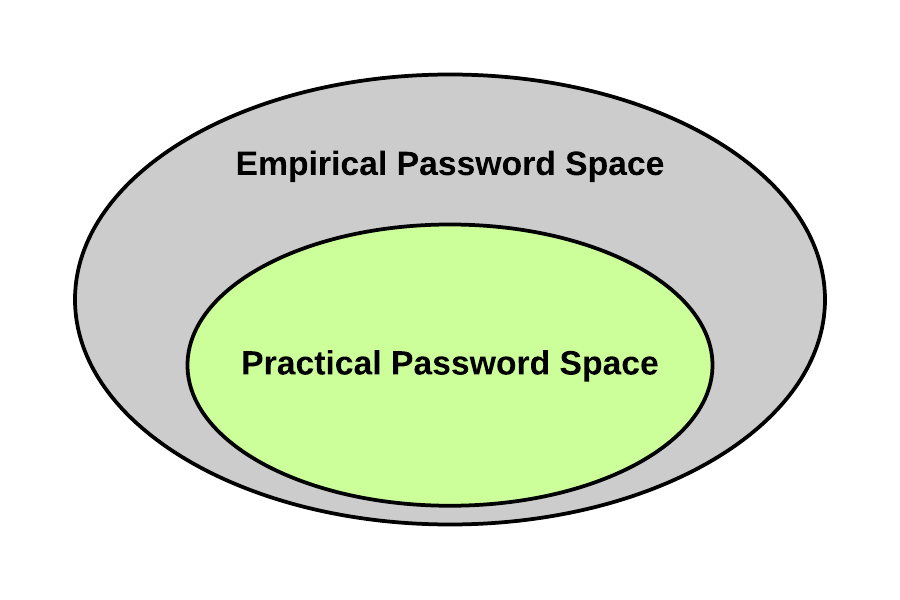
\includegraphics[scale=0.16]{pics/EmpiricalVsPractical.png}
    \end{center}
    \vspace{-20pt}
    \caption{Empirical vs. Practical Password Space}
    \vspace{0pt}
  \end{wrapfigure}

  Since a person needs to remember a password, it is normally to choose a password that are connected to you as a person in order to remember the password, causing the password to have bias. A bias can be explained as a prejudice in favor of or against one thing, person, or group compared with another, usually in a way that influence a person choice of action. The problem with many password schemes is that there are an empirical password space, but it seems that it is not the case in practice because of the biases that are often introduced, making the practical password space less than the empirical password space. In a case study of 14.000 Unix passwords, a research group found a 25\% of the passwords were in a group of words forming a dictionary of $3\times10^{6}$ words \cite{UnixPasswords}. This dictionary shows that an attacker can have a relatively high success rate with an attack, despite the fact that there a roughly $2\times10^{14}$ 8-character passwords consisting of digits, and upper case and lower case letters. Due to the limitations of human memory, useres often choose passwords which are easier to remember, causing a significant number of user-chosen password to fall into a small dictionary, e.g. practical password space \cite{Tao}. A well-designed dictionary is a tiny subset of the full password spave, e.g. theoretical password space, which further can be prioritized  according to the likelihood for a password to be chosen. It is therefore a commonly stated that the security of a password scheme is releted closely to the size of its memorable/practical password space, rather than its theoretical password space. Since psychological studies have recognized that the human brain have a superior memory for recognizing and recalling visual information, it support the statement that users are able to remember more complex graphical password form a larger password space than a alphanumeric password. Logically the attacker then have to build a bigger and more complex dictionary, thus spend more time to achieve the same success rate as for textual passwords. % Her må jeg ha noen eksempler på dictionary attacks mot grafiske passord!!!

  The graphical password scheme DAS \cite{Jermyn} was evaluating the security of their password scheme. They highlighted that there are many factors that impacts the security of a password scheme, like the statement that the users do not use a uniformal distribution of all possible passwords, using Klein's study \cite{UnixPasswords} as a argument. The fact that useres do not pick passwords uniformly is not in itself a sufficient statement to make a guessing attack successful. They try to cover the possibility for a attacker making a successful attack by making their scheme complex, and the results showed that the generated passwords was significantly harder to crack in practice than texutal passwords. The problem is that they used coputer generated passwords that will not show acutally password chosen by user. They did not analyse the security of the DAS including human factors and password biases that may could incluence the practical password space. 
  

  